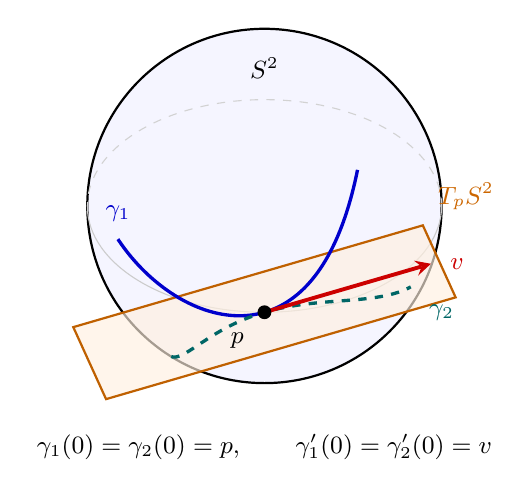
\begin{tikzpicture}[>=stealth, scale=1.25,
    x={(1.8cm,0cm)}, y={(0cm,1.44cm)}, z={(0cm,-1.08cm)}]
  % Orthographic projection of the unit sphere: (x,y,z) -> (1.8x,1.44y-1.08z).
  \draw[thick, fill=blue!4] (0,0) circle[radius=1.8cm];
  \draw[gray!35, dashed] (1.8cm,0cm) arc (0:180:1.8cm and 1.08cm);
  \draw[gray!40] (-1.8cm,0cm) arc (180:360:1.8cm and 1.08cm);
  \node[font=\small] at (0cm,1.4cm) {$S^2$};

  % A patch of the actual tangent plane z=1 at p=(0,0,1).
  \filldraw[fill=orange!12, fill opacity=0.65,
      draw=orange!75!black, thick]
    (-0.894,-0.613,1) -- (1.079,0.105,1) --
    (0.894,0.613,1) -- (-1.079,-0.105,1) -- cycle;
  \node[font=\small, text=orange!80!black, above right=2pt]
    at (0.894,0.613,1) {$T_pS^2$};

  % In a rotated tangent basis e1,e2, use
  % gamma_i(t)=t e1 +/- 0.85 t^2 e2 + sqrt(1-t^2-0.85^2 t^4) p.
  % Both lie on S^2, pass through p, and have derivative e1 at t=0.
  \draw[blue!80!black, very thick]
    plot[domain=-0.72:0.72, samples=101, variable=\t]
    ({cos(20)*\t-sin(20)*0.85*\t*\t},
     {sin(20)*\t+cos(20)*0.85*\t*\t},
     {sqrt(1-\t*\t-0.85*0.85*\t*\t*\t*\t)});
  \draw[teal!80!black, very thick, dashed]
    plot[domain=-0.72:0.72, samples=101, variable=\t]
    ({cos(20)*\t+sin(20)*0.85*\t*\t},
     {sin(20)*\t-cos(20)*0.85*\t*\t},
     {sqrt(1-\t*\t-0.85*0.85*\t*\t*\t*\t)});

  % Labels sit beside separated portions of the curves.
  \node[font=\small, text=blue!80!black, above=3pt]
    at (-0.827,0.168,0.537) {$\gamma_1$};
  \node[font=\small, text=teal!80!black, below right=3pt]
    at (0.827,-0.168,0.537) {$\gamma_2$};

  \draw[->, red!80!black, line width=1.4pt]
    (0,0,1) -- ({cos(20)},{sin(20)},1)
    node[right=3pt, font=\small] {$v$};
  \fill (0,0,1) circle[radius=2pt];
  \node[font=\small, below left=4pt] at (0,0,1) {$p$};
  \node[font=\small, align=center] at (0cm,-2.45cm)
    {$\gamma_1(0)=\gamma_2(0)=p,\qquad
       \gamma_1'(0)=\gamma_2'(0)=v$};
\end{tikzpicture}
